\chapter{Introduction\label{cha:introduction}}
%% \ifdraft only shows the text in the first argument if you are in draft mode.
%% These directions will disappear in other modes.
\ifdraft{State the objectives of the exercise. Ask yourself:
  \underline{Why} did I design/create the item? What did I aim to
  achieve? What is the problem I am trying to solve?  How is my
  solution interesting or novel?}{}

In the year $2017$ the approximate amount of adults with diabetes was 425-million people \cite{Intro_FactsandFigures}, this number is 
projected to rise to $629$-million people by the year $2045$. The rate of people that are diagnosed with diabetes 
is 1 in every 2. Secondly of all people with diabetes 1 in every 3 develop diabetic retinopaty (DR)\cite{Intro_DiabetesRate}.

\textit{Diabetic retinopathy} is a symptom of both type 1 and type 2 diabetes and is now the leading cause of blindness amongst adults today. DR is 
diagnosed by two major technologies, firstly there is the fundus imaging method, where a photograph is taken of the fundus (back) 
of the patients eye, an example of this can be seen in Figure \ref{fig:fundus-image1}. Secondly ophthalmologists examine 
Optical Choerence Tomography (OCT) scans of human retina, an example of this can be seen in Figure \ref{fig:oct-retina1}. 
The work in this paper does not focus on the latter. The diagnosis of DR is costly and as the statistic indicate 
the amount of work is going to increase.

\begin{figure}[h]
  \centering
  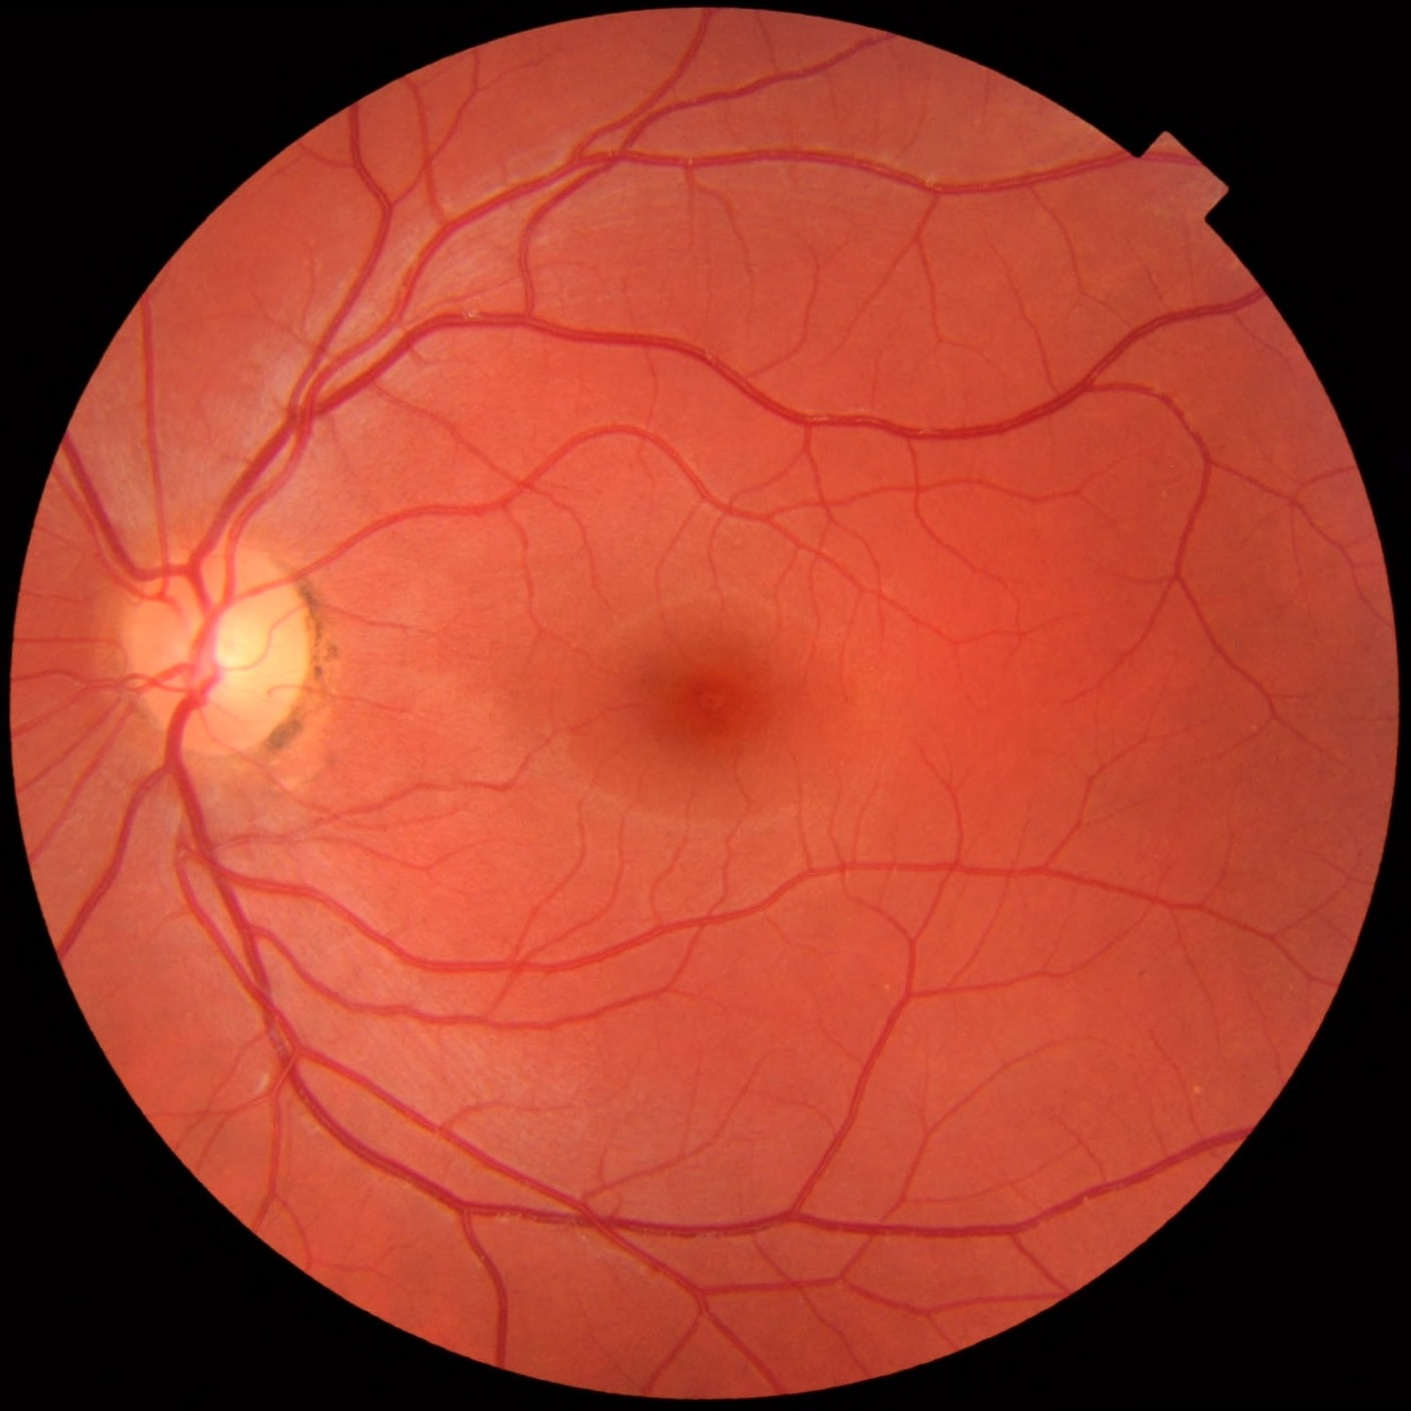
\includegraphics[width=.3\linewidth]{../graphics/fundus_image1.jpg}
  \caption{Example of Fundus image}
  \label{fig:fundus-image1}
\end{figure}
\begin{figure}[h]
  \centering
  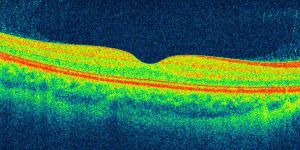
\includegraphics[width=.5\linewidth]{../graphics/oct_fundus.png}
  \caption{Example of OCT on Retina}
  \label{fig:oct-retina1}
\end{figure}

Patients that have DR are grouped into four different stages\cite{Intro_FourStages}:

1. \textit{Mild Nonproliferative Retinopathy} - This is the earliest stage of diabetic retinopathy, and it’s characterized by balloon-like swelling in the retina’s blood vessels. These are called microaneurysms, and these vessels can leak into the eye.

2. \textit{Moderate Nonproliferative Retinopathy} - During this stage, the blood vessels nourishing the retina swell and may even become blocked. This can contribute to diabetic macular edema (DME) which is a build-up of fluid in the macula region of the retina.

3. \textit{Severe Nonproliferative Retinopathy} -  At this stage, an increasing number of blood vessels nourishing the eye have become blocked. As a result, the retina is signaled to grow new blood vessels.

4. \textit{Proliferative Diabetic Retinopathy} - This is the final stage of diabetic retinopathy. New blood vessels proliferate, growing inside the retina and into the vitreous gel, which is the fluid that fills the eye. Because these blood vessels are delicate, they may begin to leak and bleed. As a result, scar tissue may form, causing retinal detachment, the pulling away of the retina from underlying tissue. Retinal detachment may cause spotty vision, flashes of lights, or severe vision loss.

Generally without intervention patients advance from one stage to the next eventually leading 
to permanent vision impairment, however with intervention by an ophthalmologist this advancement 
can be prevented \cite{Intro_StageAdvancement}. 

This paper focuses on applying machine learning methods to patient information and Fundus images of those 
patients to assess the likelyhood (risk) of those patients DR developing into SDR.

In this paper we will apply machine learning methods to patients information and fundus images of patients 
that has been collected a period of time to examine a patiens likelyhood to advance from one stage 
of DR to the next, attempting to predict the timeline the patient has to seek medical help. 

\section{Machine learning methods in Ophthalmology}

Applying machine learning to fundus images and patient information has been done before very successfully 
researchers\cite{Intro_googleDeepmind}, this work generally focuses on applying image recognition on 
the images to identify which stage of DR the eye has reached. 

\section{Background}
\ifdraft{Provide background about the subject matter (e.g. How was morse code
developed?  How is it used today?). 
This is a place where there are usually many citations.
It is suspicious when there is not. 
Include the purpose of the different equipment and your design intent. 
Include references to relevant scientific/technical work and books.}

Applying statistics to medical data in order to better understand a patients evolution from DR to SDR 
has been done previously by a company called RetinaRisk, a significant contributor to this paper, but 
RetinaRisk's solution does not apply machine learning but a specialists field knowledge and a handcrafted 
formula. RetinaRisks formula has been used to significantly reduce costs to health organizations as 
when patients following their recommendations for doctor checkups come in less often but at time that 
are more critical. im just writing something so that it looks like I'm writing something
